\documentclass[norsk,a4paper,12pt]{article}
\usepackage[utf8]{inputenc}
\usepackage{graphicx} %for å inkludere grafikk
\usepackage{verbatim} %for å inkludere filer med tegn LaTeX ikke liker
\usepackage{tabularx}
\usepackage{booktabs}
\usepackage{amsmath}
\usepackage{float}
\usepackage{color}
\usepackage{listings}
\usepackage{hyperref}
\usepackage{amsmath}
\usepackage{tikz}
\usepackage{physics}

\lstset{language=c++}
\lstset{basicstyle=\small}
\lstset{backgroundcolor=\color{white}}
\lstset{frame=single}
\lstset{stringstyle=\ttfamily}
\lstset{keywordstyle=\color{red}\bfseries}
\lstset{commentstyle=\itshape\color{blue}}
\lstset{showspaces=false}
\lstset{showstringspaces=false}
\lstset{showtabs=false}
\lstset{breaklines}
\lstset{postbreak=\raisebox{0ex}[0ex][0ex]{\ensuremath{\color{red}\hookrightarrow\space}}}
\usepackage{titlesec}

\setcounter{secnumdepth}{4}
\usetikzlibrary{through,calc,er,positioning}

\titleformat{\paragraph}
{\normalfont\normalsize\bfseries}{\theparagraph}{1em}{}
\titlespacing*{\paragraph}
{0pt}{3.25ex plus 1ex minus .2ex}{1.5ex plus .2ex}


\title{FYS4411 - Computational Physics II\\\vspace{2mm} \Large{Project 2}}
\author{\large Dorthea Gjestvang\\ Even Marius Nordhagen}
\date\today
\begin{document}

\maketitle

\begin{itemize}
\item Github repository containing programs and results: \\\url{https://github.com/evenmn/FYS4411/tree/master/Project%202}
\end{itemize}

\begin{abstract}
Abstract
\par 

\end{abstract}

\newpage

\tableofcontents

\newpage

\section{Introduction} \label{sec:Introduction}


\section{Theory} \label{sec:Theory}
\subsection{Presentation of potential} \label{sec:Presentation_of_potential}
In this project, we simulate a system of $P$ electrons trapped in a harmonic oscillator potential, with a Hamiltonian given by

\begin{equation}
\label{eq:Hamiltonian}
\hat{H} = \sum_{i=1}^{P} (-\frac{1}{2} \nabla_i^2 + \frac{1}{2} \omega^2 r_i ^2) + \sum_{i<j} \frac{1}{r_{ij}} 
\end{equation}

where $\omega$ is the harmonic oscillator potential and  $r_i = \sqrt{x_i^2 + y_i^2}$ is the position of electron $i$. The term $\frac{1}{r_{ij}}$ is the interacting term, where $r_{ij} = |r_i - r_j|$ is the distance between a given pair of interacting electrons. Natural units have been used, such that $\hbar = c = m_e = e = 1$.

Since electrons are fermions, we need an antisymmetric wavefunction under exchange of two coordinates, and we need to take the Pauli principle into account. A Slater determinant is therefore needed for multiple fermions to ensure that the total wavefunction is antisymmetric. In this project we will study particles in the ground state only, and according to the Pauli principle we can in this case study a maximum of two particles with spin $s=\pm 1/2$. The slater determinant for two particles read
\begin{equation}
\Psi_T=
\begin{vmatrix}
\Phi_1(\boldsymbol{r}_1) & \Phi_2(\boldsymbol{r}_1)\\
\Phi_1(\boldsymbol{r}_2) & \Phi_2(\boldsymbol{r}_2)
\end{vmatrix}
=\Phi_1(\boldsymbol{r}_1)\Phi_2(\boldsymbol{r}_2)-\Phi_2(\boldsymbol{r}_1)\Phi_1(\boldsymbol{r}_2)
\end{equation}
where $\Phi_i(\boldsymbol{r})$ is the single particle wave function (SPF) of state $i$. This contains a spatial part and a spin part, and we assume that it can be splitted up such that the spin part takes the antisymmetry property and does not affect the energy. Therefore we only need a symmetric spatial part to calculate the energies.

\subsection{Solving this with machine learning}
When solving a system of particles as the one described in the previous system with Variational Monte Carlo, as described in \cite{Nordhagen}, we would need an anzats for the wave function, where we use our physical intuition to create the form of a wave function with different variational parameters, and then let it be up to the computer to find the optimal parameters through a minimization method. However, this method is only as good as the physical intuition; if the form of the wave function is unrealistic, the results will be the same
\par 
\vspace{3mm}
This challenge can be mended by using machine learning. There are several different types of machine learning systems, and the one we will present and utilize in this project has the ability to learn and sample from a probability distribution. This is perfect for quantum mechanical problems, as we know from quantum mechanics the wave function $\Psi$ is nothing more than a probability denisty, giving that $\Psi^2$ is a probability distribution that says something about where a given particle most probabliy can be found. As we are solely interested in the energy of the two-fermion system, and not the exact wave function, the fact that the machine learning program does not explicitly give the wave function is therefore of no consequence. We still have to give some guidelines for the form of the probability distribution, but the machine learning program can sample from a larger variety of probability distributions compared to the form used in VMC.

\subsubsection{Machine learning}
With the goal of solving the quantum mechanical system presented in section \ref{sec:Presentation_of_potential} in mind, we should start by explaining what machine learning is. Machine learning is the idea that a computer can be trained to learn to yield certaint outputs, without directly being told exactly what to give. Examples on this is pattern recognizion, where the computer first is shown for example pictures of wolves and huskies. After training the computer on pictures where the computer sees huskies and wolves and is told the correct answer, it should after a sufficiently long training period, be able to recognize huskies and wolves by itself. 
\par 
\vspace{3mm}
The example described above is what we call supervised learning, where the correct output answer is known during the training program. A machine learning program could also be unsupervised, where the correct answer is unknown, or based on reinforcement learning, where the the program learns by conducting trial-and-error experiments. 
\par 
\vspace{3mm}

\subsubsection{Neural network}

 This sound amazing, and maybe even impossible. Therefore the question now is: how to program computers to learn, just like humans? The answer is, fittingly, that we should make the program run like the the human brain by implementing what is called a neural network. Inspired by neurons in the human brain, a neural network is a programmed network of variables, called nodes, that comminucate in a given manner. Each node preforms a simple process: based on the input it receives, and how that input is weighted, it decides wheter or not to fire. The mathematical model of an example of a neural node was presented by McCulloch and Pitts in 1943 \cite{Marsland}, shown in figure \ref{fig:neuron}, where the input is mared $x_i$, the weights deciding how much the input should count is $W_i$, and the output from the node based on $x_i$ and $W_i$ is called h. 

 \begin{figure} [H]
 	\centering
 	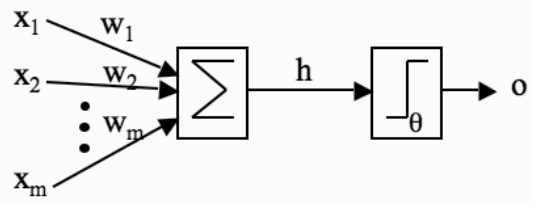
\includegraphics[scale=0.6]{plots/neuron.png}
 	\caption{McCullochs and Pitts' model of neutrons visualized. Image reproduced from \cite{Marsland} }
 	\label{fig:neuron}
 \end{figure}

The neutrons are arranged in layers in the neural network, one visible layer that receives the input, and up to several hidden layers. The layers are arranged such that the output values from the visible nodes is the input values of the visible nodes. The nodes can also have bias values, that shift the output value $h$ with a ceirtan number, and the nodes in different layers can be connected in different ways.  An example of a neural network with two layers is shown in figure \ref{fig:neural_network}.

 \begin{figure} [H]
	\centering
	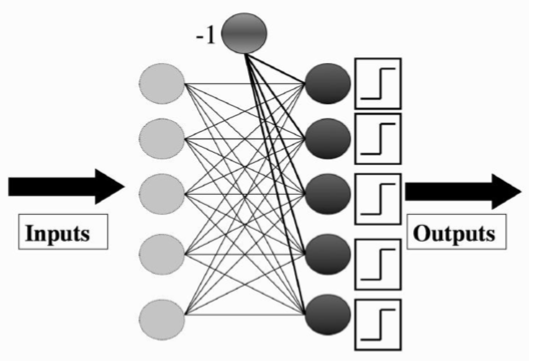
\includegraphics[scale=0.5]{plots/neural_network.png}
	\caption{An example of a neural network with one visible and one hidden layer of nodes, and with bias $-1$ on the hidden nodes. Image reproduced from \cite{Marsland} }
	\label{fig:neural_network}
\end{figure}

The idea behind machine learning is that the weights $W_i$, that decides how much a node puts emphazis on a given input, can be changed, and thus change the system's response to the same input. We will explain with the example from earlier, with huskies and the wolves: first, the program are shown pictures of wolves and huskies, and it is told the correct answer. The weights $W_i$ are then updated such that when a husky is shown, the output "husky" is generated, and the same for wolves. After a sufficiently long training period, the program's weights are optimalized for recognizing wolves and huskies. When shown a picture, the program should then by itself be able to determine wheter it is a wolf or a husky that it sees. 

\subsubsection{Restricted Boltzmann Machines}
There are plenty of ways to put together a neural network, as one can modify the number of nodes and layers, the bias, and also which nodes that are allowed to communicated. In this project, we will be using the so-called Restricted Boltzmann Machine (RBM). It is a two-layer network. The reason why it is named "restrictive" is that there are no connections between nodes in the same layer, but every node in the previous layer is connected to all the nodes in the next layer. The RBM can learn to draw samples from a probability distribution, which is just what we want in our project. In addition, we want to use a Gaussian-Binary RBM, where the hidden nodes have binary values, while the positions of the particles can take continous values, as they are, in fact, positions. 

The joint probability distribution is known from statistical mechanics,
\begin{equation}
F(\boldsymbol{X},\boldsymbol{H})=\frac{1}{Z}e^{-\beta E(\boldsymbol{X},\boldsymbol{H})}
\end{equation}
where we set $\beta=1/kT=1$ and $Z$ is the partition function, which can be ignored since it will vanish anyway. 

The system energy of a Gaussian-Binary RBM is given by
\begin{equation}
E(\boldsymbol{X},\boldsymbol{H})=\sum_{i=1}^{M}\frac{(X_i-a_i)^2}{2\sigma_i^2}-\sum_{j=1}^Nb_jH_j-\sum_{i,j=1}^{M,N}\frac{X_iW_{ij}H_j}{\sigma_i^2}
\end{equation}
(Hinton 2010). 

By setting $\Psi = F(\boldsymbol{X},\boldsymbol{H})$, we know have a general form of the probability distribution. In equation \ref{eq:wf_form} the form of the wave function is shown, when we have used that we have $M$ visible nodes and $N$ hidden nodes, and that the hidden nodes should take binary values. 

\begin{equation}
\label{eq:wf_form}
	\Psi = \frac{1}{Z} e^{\sum_i^M \frac{(X_i - a_i)^2}{2\sigma^2}} \prod_j^N (1+ e^{b_j + \sum_iM \frac{X_i W_{ij}}{\sigma^2}})
\end{equation}

\subsection{Energy calculation}
We want to calculate the energy of the two-fermion system, given the wave function described in \ref{eq:wf_form}. As explained in \cite{Nordhagen}, the energy of the system is the expectation value of the Hamiltonian, but this is hard to compute directly. 

\begin{equation}
E_L(\vec{r})=\frac{1}{\Psi_T(\vec{r})}\hat{H}\Psi_T(\vec{r}).
\label{eq:Local_energy}
\end{equation}

By defining the local energy given in equation \ref{eq:Local_energy}, the energy can be expressed as equation \ref{eq:MC_energy}, and this can be solved with a Monte Carlo loop.

\begin{equation}
\label{eq:MC_energy}
E = \int | \Psi_T^2| E_L d\vec{r}
\end{equation}

\subsubsection{Exact energy for non-interacting case}

The wave function of one electron in a two-dimensional harmonic oscillator is given by

\begin{equation}
	\label{eq:one_e_wf_ho}
	\phi_{n_x, n_y} = A H_{nx} \sqrt{\omega} x H_{ny} \sqrt{\omega} y e^{-\frac{\omega(x^2 + y^2)}{2}}
\end{equation}

where $H_{nx} \sqrt{\omega} x$ is the Hermite polynomials and A is the normalization constant, and $n_x$ and $n_y$ are the principal quantum numbers. If we denote $\phi_1$ the spatial wave function for the first electron, and $\phi_2$ the spatial wave function for the second electron, then the total spatial wave function for the two-particle system is $\phi_1 \phi_2$. As explained in section \ref{sec:Presentation_of_potential}, the spin wave functions are anti-symmetric, and therefore it is fine that the spatial wave function is symmetric.

For a one-electron system the energy can be shown to take the value 

\begin{equation}
	H \ket{\phi_1} = E_1 \ket{\phi_1} = \omega(n_{x,1} + n_{y,1} + 1) \ket{\phi_1} \quad  \rightarrow E_1 = \omega(n_x + n_y + 1)
\end{equation}
where we have used natural units, and all the energies are given in atomic units a.u.

When calculating the energy for the two-electron system we then get the following

\begin{equation}
	H \ket{\phi_1 \phi_2} = \ket{H \phi_1 } \ket{\phi_2} + \ket{\phi_1} \ket{H \phi_2} = E_1 \ket{\phi_1 \phi_2} + E_2 \ket{\phi_1 \phi_2} 
\end{equation}

For the ground state $n_x = n_y = 0$, $E_1 = E_2 = \omega$ and therefore the ground state energy is simply $E_1 + E_2 = 2\omega$. 

For the non-interacting case with $\omega=1$ it is known the ground state energy is 3 a.u. \cite{Project2}. 

\subsection{Onebody density}

\subsection{Scaling}

\subsection{Error estimation}
As a physicist one should always be sceptical to measurements presented without an estimation of the uncertainties. When someone says they have measured their height to be 1.90 cm, is the uncertainty $\pm 1 cm$ or $\pm 10 cm$? If they used $\pm 1 cm$, we have a fairly good idea of the height of the person, but if it is $\pm 10 cm$, we do not really know anything about the real height of the person. 
\par 
\vspace{3mm}
The error in a measurement is the difference between the true value of the mesurand, $x$, and the mesured value $x_i$:

\begin{equation}
	error = x - x_i
\end{equation}

However, the true value $x$ is rarely known. When $x$ is not known, it is thus impossible to give the error in the measurement. We must therefore be content with providing estimates of the error. It is common to give this uncertainty as the standard deviation $\sigma$; when preforming a mesurement n times, such that we have n measured points $x_1, .., x_n$ where the average value is $ \langle x \rangle $, then the standard deviation is defined as

\begin{equation}
\sigma_{\theta} =  \sqrt{\frac{1}{n} \sum_{k=1}^n (x_i - \langle x \rangle)^2}
\end{equation}

When giving the uncertainty, one writes $x_i \pm \sigma$, where $\sigma$ is so that $\approx 68 \%$ of the measured values lies withing the interval $\pm \sigma$. 

There are different kinds of sources of error when conducting computer experiments. Systematic errors originate from faults in the theory used in the experiment, and this might give consistently wrong results. Systematic errors are hard to handle, as one might get seemingly good looking results. One way to avoid systematic results are to benchmark the code with either experimental results, or with other's computer simulation results. \par 
\vspace{3mm}
Another source of error is the statistical error, which is based on how many measurements you have done. In the example with the height measurement in the beginning of this section, if the experimentalist only measured the height one time, we can be fairly certain that this is not the true value of the person. If they, however, repeated the same measurement several times and then maybe used the average as the estimate of the mesurand, we can be more confident that they have a better estimate, compared to when they only used one point. A common way to estimate the statistical uncertainty is with equation \ref{eq:variance_simplified}.

\begin{equation}
\label{eq:variance_simplified}
\sigma^2 \approx \langle x^2 \rangle - \langle x \rangle^2
\end{equation}

However, as explained in \cite{Nordhagen}, this does not account for the covarinace between measurements. This leads to equation \ref{eq:variance_simplified} being an underestimation of $\sigma^2$, and is thus more a guideline for the size of the uncertainty, more than an actual estimate of it. Luckily, there are computational methods that can calculate $\sigma^2$ with the covariance contribution included. The method used in this project is the blocking method, presented in section \ref{sec:Blocking}.

\section{Method}

\subsection{Variational Monte Carlo}
The Variational Monte Carlo method, often referred to as VMC, is a method in computational physics. The goal of VMC is to approximate the ground state energy of a quantum mechanical system by using the variational principle. The variational principle says that for any given trial wave function $\Psi_T$, the energy $E$ given this $\Psi_T$ is always more than or equal to the ground state energy $E_0$ of the system:

\begin{equation}
	\label{eq:variational_method}
	E = \frac{\bra{\Psi_T}H \ket{\Psi_T}}{\braket{\Psi_T}} \geq E_0
\end{equation} 

In VMC, the user inputs a trial wave function for the quantum mechanical system. Over a Monte Carlo loop, the particles in the system are moved randomly, and for each proposed move, the new position of the particle is accepted or rejected depending on if the new position is more probable according to $\Psi_T$, compared to the previous position. For the ground state wave function, the position which yields a minimum in the energy of the quantum mechanical system is the most probable position. The result is therefore that the particles in the system are moved towards lower energies. When the method has converged, the energy $E$ is an upper estimate of the true ground state energy $E_0$. If $\Psi_T$ in addition is the true ground state wave function, then $E=E_0$. 

\subsection{Metropolis algorithm}
Above, we described that the VMC method had to reject or accept proposed moves of the particles in the system. The task of handeling this is often left up to the Metropolis algorithm. The Metropolis algorithm uses the theory that the probability of a system to transition from a state $i$ to state $j$ is given by

\begin{equation}
W_{i\rightarrow j} = T_{i \rightarrow j}\cdot A_{i \rightarrow j}
\end{equation}

where $T_{i \rightarrow j}$ is the transition probability and $A_{i \rightarrow j}$ is the acceptance probability. If we denote the probability for being in a given state for $p$, and then look at the transition from a state $i$ to a state $j$ and back again, then it can be shown that we obtain the following relation between the transition and acceptance probabilities \cite{Nordhagen}:

\begin{equation}
\label{eq:metropolis_acceptance}
\frac{A_{j\rightarrow i}}{A_{i\rightarrow j}}=\frac{p_iT_{i\rightarrow j}}{p_jT_{j\rightarrow i}} = w
\end{equation}

As the Metropolis algorithm's job is to evaluate probable moves between states, the expression in equation \ref{eq:metropolis_acceptance} is used as the acceptance criteria. Thus the ratio $\frac{A_{j\rightarrow i}}{A_{i\rightarrow j}}$ describes if the system is more likely to move one way or the other. There are several methods that can be used for accepting and rejecting the moves, and these use different expressions for $T$ and $p$ in equation \ref{eq:metropolis_acceptance}. In this project, we will study the brute force and the Hastings sampling algorithms.

\subsubsection{Brute force}
The brute force got is name because when proposing and accepting moves, the algorithm does so without "thinking" which way the system will most probably move. A random particle with position $\vec{R}$ is chosen, and its new position $\vec{R}_{new}$ is proposed at random as follows:

\begin{equation}
\boldsymbol{R}_{new} = \boldsymbol{R} + r\cdot \text{step}.
\end{equation}

where $r$ is a random number and $step$ is the steplength.
\par 
\vspace{3mm}
The brute force algorithm does not concider the transitions probabilities, and simply puts $T_{i\rightarrow j} = T_{j\rightarrow i}$. To check the probability of a system being found in a given state, it uses $p(\vec{R})=|\Psi_T(\vec{R})|^2$ for both position, such that the probability $w$ for the transition is given by

\begin{equation}
w=\frac{P(\vec{R}_{new})}{P(\vec{R})}=\frac{|\Psi_T(\vec{R}_{new})|^2}{|\Psi_T(\vec{R})|^2}.
\end{equation}

A random number $r \in [0,1]$ is then drawn, and compared to $w$. If $w$ is larger than $r$, then the new position is accepted, and if not, the move is rejected and the particle is moved back to its original position:

\begin{equation}
\text{New position: }
\begin{cases} 
\text{accept} & \text{if}\quad w > r \\
\text{reject} & \text{if}\quad w \leq r.
\end{cases}
\end{equation}

This way, the algorithm will over many iterations move the particles towards the most probable state.


\subsubsection{Metropolis-Hastings}
also known as importance sampling
\subsection{Gibbs sampling}

\subsection{Gradient descent}
We use stochastic gradient descent to update the weights in order to minimize the local energy. The process itself is quite similar to that one typically used in Variational Monte Carlo (VMC) where the weights are our variational parameters, but compared with a normal VMC we have a lot more parameters to vary. The updating algorithm for updating the variational parameter $\alpha_i$ goes as
\begin{equation}
\alpha_i^+=\alpha_i-\eta d\alpha_i
\end{equation}
where the gradient of the local energy with respect to parameter $\alpha_i$ is
\begin{equation}
d\alpha_i=\frac{\partial\langle E_L\rangle}{\partial \alpha_i}=2\bigg(\Big\langle E_L\frac{1}{\Psi}\frac{\partial\Psi}{\partial\alpha_i}\Big\rangle-\Big\langle E_L\Big\rangle\Big\langle\frac{1}{\Psi}\frac{\partial\Psi}{\partial\alpha_i}\Big\rangle\bigg)
\end{equation}
where $\eta$ is the learning rate. We need to do this for all the parameters, and for our purposes it is convenient to vectorize the gradient such that $d\boldsymbol{a}$ and $d\boldsymbol{b}$ are vectors and $d\boldsymbol{W}$ is a matrix. The gradients to implement are
\begin{equation}
d\boldsymbol{a}=\frac{1}{\Psi}\frac{\partial\Psi}{\partial\boldsymbol{a}}=\frac{\boldsymbol{X}-\boldsymbol{a}}{\sigma^2}
\end{equation}
\begin{equation}
d\boldsymbol{b}=\frac{1}{\Psi}\frac{\partial\Psi}{\partial\boldsymbol{b}}=
\end{equation}

\subsubsection{Adaptive stochastic gradient descent}
A problem with the standard stochastic gradient descent method is that it will either converge fast, but the precision is poor, or the precision is good, but it converges slowly. To avoid this problem, we want a large learning rate when the energy is far from converging and a small learning rate when the energy converges. 

\subsection{Blocking method} \label{sec:Blocking}

\section{Code}
\subsection{Structure}
\subsection{Implementation}

\section{Results} \label{sec:Results}

\section{Discussion} \label{sec:Discussion}

\section{Conclusion} \label{sec:Conclusion}

\newpage

\section{Appendix A - Local energy calculations} \label{sec:appendix_A}
The energy can be calculated by introducing a local energy, where the acerage local energy goes to the true energy with a sufficient amount of samples. This local energy can be splitted up in a kinetic part, a part from the harmonic oscillator potential and a interacting part,
\begin{equation}
E_L=\sum_{k=1}^{M}(E_{\text{KIN},k} + E_{\text{EXT},k})+E_{\text{POT}}.
\end{equation}
As discussed in \cite{Nordhagen}, the kinetic part can be expressed as
\begin{align}
E_{\text{KIN},k}&=\frac{1}{\Psi_T}\nabla_k^2\Psi_T\\
&=(\nabla_k\ln\Psi_T)^2+\nabla_k^2\ln\Psi_T
\end{align}
where we have used that
\begin{equation}
\frac{1}{\Psi_T}\nabla_k\Psi_T=\nabla_k\ln\Psi_T.
\end{equation}

\begin{equation}
\frac{\partial}{\partial X_k}\ln\Psi_T=-\frac{X_k-a_k}{\sigma^2}+\sum_{j=1}^{N}\frac{W_{kj}}{\sigma^2}\text{Logistic}(v(j))
\end{equation}
\begin{equation}
\frac{\partial^2}{\partial X_k^2}\ln\Psi_T=-\frac{1}{\sigma^2}+\sum_{j=1}^{N}\frac{W_{kj}^2}{\sigma^4}\text{Logistic}^2(v(j))e^{v(j)}
\end{equation}
where 
\begin{equation}
\text{Logistic}(x)=\frac{1}{1+e^x}
\end{equation}
and
\begin{equation}
v(j)=b_j+\sum_{i=1}^{M}\frac{X_iW_{ij}}{\sigma^2}.
\end{equation}
Thus the local energy can be expressed as
\begin{align}
E_L&=\sum_{i=1}^{N}\frac{\boldsymbol{W}_{*i}^T\boldsymbol{W}_{*i}}{\sigma^4}\text{Logistic}^2\big(v(i)\big)+\\
&\phantom{=}\sum_{i,j=1}^{N,N}\frac{\boldsymbol{W}_{*i}^T\boldsymbol{W}_{*j}}{\sigma^4}\text{Logistic}\big(v(i)\big)\text{Logistic}\big(v(j)\big)-\\
&\phantom{=}2\sum_{i=1}^N\frac{\boldsymbol{W}_{*i}^T(\boldsymbol{X}-\boldsymbol{a})}{\sigma^4}\text{Logistic}(v(i))+\\
&\phantom{=}\frac{(\boldsymbol{X}-\boldsymbol{a})^T\cdot(\boldsymbol{X}-\boldsymbol{a})}{\sigma^4}-\frac{1}{\sigma^2}+\boldsymbol{X}^T\boldsymbol{X}+E_{\text{INT}}
\end{align}



\newpage
\section{References}

\begingroup
\renewcommand{\section}[2]{}
\begin{thebibliography}{}
	\bibitem{MHJ15}
	Morten Hjorth-Jensen.
	Computational Physics 2: Variational Monte Carlo methods, Lecture Notes Spring 2018.
	Department of Physics, University of Oslo,
	(2018).
	\bibitem{Marsland}
	S. Marsland, \emph{Machine Learning: An algorithmic Perspective, Second edition} (2015)
	\bibitem{Nordhagen}
	 D. Gjestvang, E. M. Nordhagen \emph{Computational Physics II: Project 1} (2018)
	 \bibitem{Project2}
	 V. Flugsrud and M. Hjort-Jensen
	 Project 2, The restricted Boltzmannn machine applied to the quantum many body problem. Deadline June 1
	 Department of Physics, University of Oslo,
	 (2018).
	
	
\end{thebibliography}
\endgroup

\end{document}
